\documentclass[12pt]{article}
\usepackage[utf8]{inputenc}
\usepackage[T1]{fontenc}
\usepackage{lmodern}

\usepackage{tikz}

\usetikzlibrary{shapes,arrows,positioning}

\tikzset{basic/.style={draw,fill=white!20,text width=1em,text badly centered}}
\tikzset{commit/.style={basic,circle}}
\tikzset{arrow/.style={draw,minimum height=3cm,line width=0.5mm}}
\tikzset{tag/.style={rectangle,draw,anchor=text,inner sep=2.5mm,fill=teal!50}}
\tikzset{branch/.style={rectangle,draw,anchor=text,inner sep=2.5mm,fill=green!50}}
\tikzset{msg/.style={rectangle,draw,anchor=text,inner sep=2.5mm,node distance=1.0cm,rounded corners=0.25cm}}

\begin{document}


  \centering
  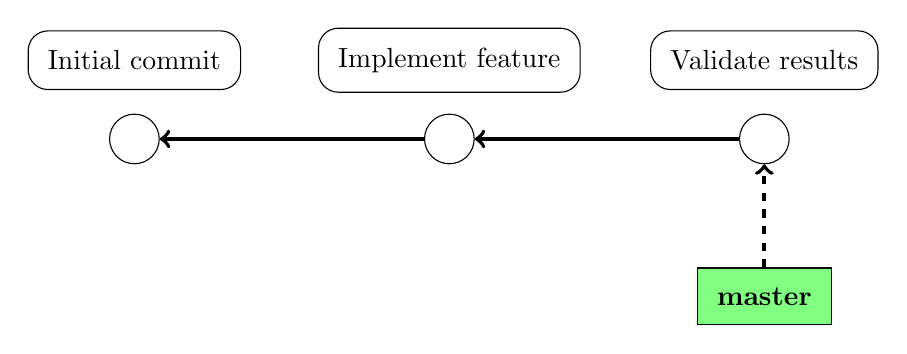
\begin{tikzpicture}[node distance=4.0cm,auto]
    \node[commit] (c1) {\quad};
    \node[commit,right of=c1] (c2) {\quad};
    \node[commit,right of=c2] (c3) {\quad};

     \node[branch,below of=c3,node distance=2.0cm] (master) {\textbf{master}};

     \node[msg,above of=c1] (m1) {Initial commit};
     \node[msg,above of=c2] (m2) {Implement feature};
     \node[msg,above of=c3] (m3) {Validate results};

        \path[arrow, <-] (c1) -- (c2);
        \path[arrow, <-] (c2) -- (c3);
        \path[arrow,dashed,->] (master) -- (c3);
  \end{tikzpicture}

\clearpage

  \centering
  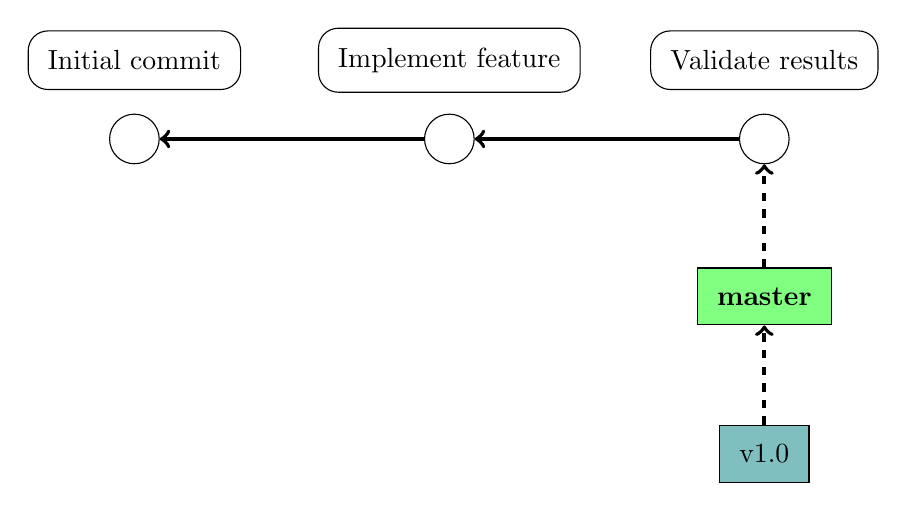
\begin{tikzpicture}[node distance=4.0cm,auto]
    \node[commit] (c1) {\quad};
    \node[commit,right of=c1] (c2) {\quad};
    \node[commit,right of=c2] (c3) {\quad};

     \node[branch,below of=c3,node distance=2.0cm] (master) {\textbf{master}};
     \node[tag,below of=master,node distance=2.0cm] (vone) {v1.0};

     \node[msg,above of=c1] (m1) {Initial commit};
     \node[msg,above of=c2] (m2) {Implement feature};
     \node[msg,above of=c3] (m3) {Validate results};

        \path[arrow, <-] (c1) -- (c2);
        \path[arrow, <-] (c2) -- (c3);
        \path[arrow,dashed,->] (master) -- (c3);
        \path[arrow,dashed,->] (vone) -- (master);
      \end{tikzpicture}
      
      \clearpage
      
  \centering
  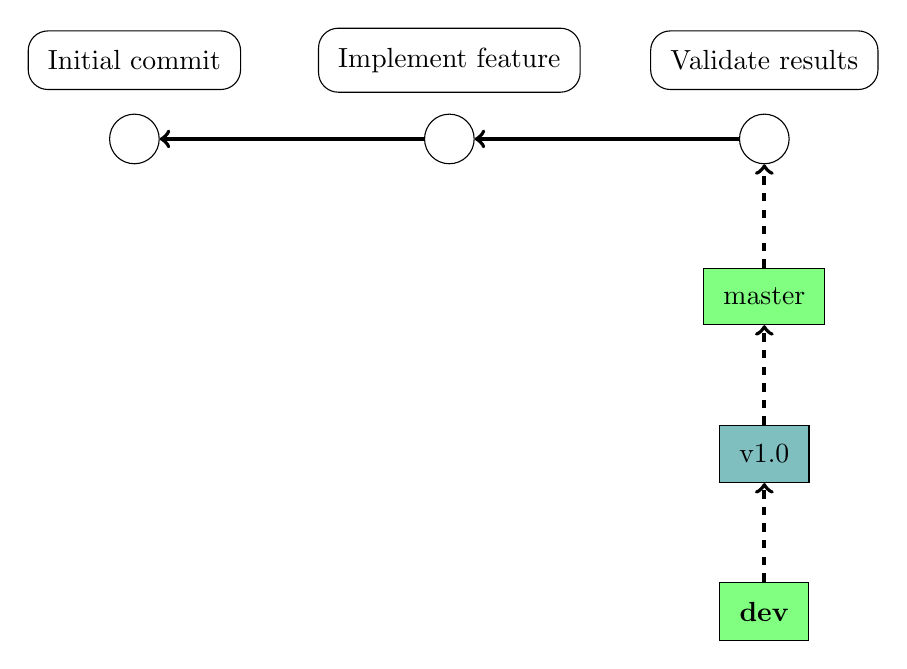
\begin{tikzpicture}[node distance=4.0cm,auto]
    \node[commit] (c1) {\quad};
    \node[commit,right of=c1] (c2) {\quad};
    \node[commit,right of=c2] (c3) {\quad};

     \node[branch,below of=c3,node distance=2.0cm] (master) {master};
     \node[tag,below of=master,node distance=2.0cm] (vone) {v1.0};
     \node[branch,below of=vone,node distance=2.0cm] (dev) {\textbf{dev}};

     \node[msg,above of=c1] (m1) {Initial commit};
     \node[msg,above of=c2] (m2) {Implement feature};
     \node[msg,above of=c3] (m3) {Validate results};

        \path[arrow, <-] (c1) -- (c2);
        \path[arrow, <-] (c2) -- (c3);
        \path[arrow,dashed,->] (master) -- (c3);
        \path[arrow,dashed,->] (vone) -- (master);
        \path[arrow,dashed,->] (dev) -- (vone);
  \end{tikzpicture}

  \clearpage

  \centering
  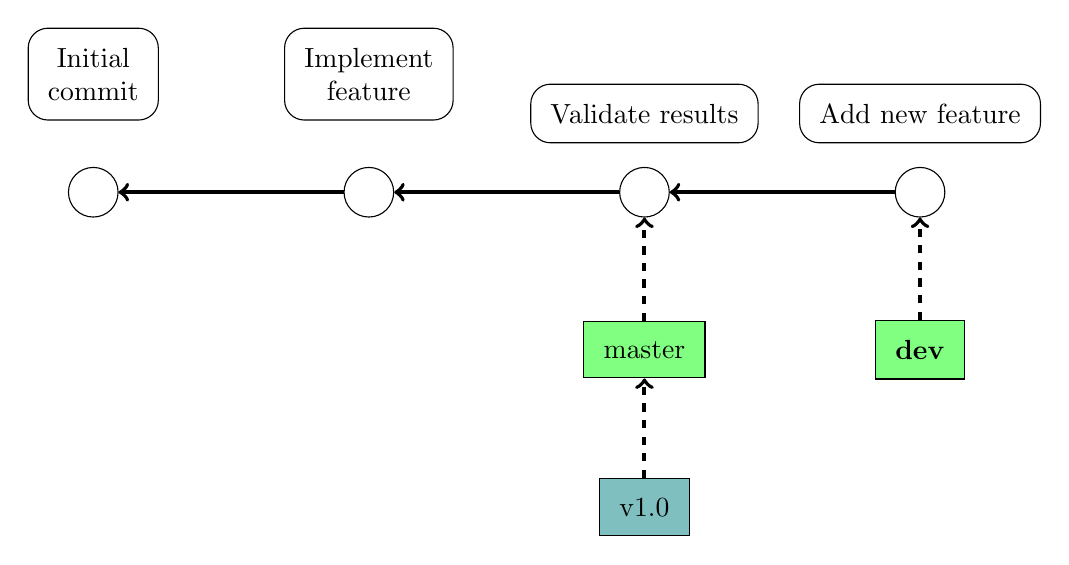
\begin{tikzpicture}[node distance=3.5cm,auto]
    \node[commit] (c1) {\quad};
    \node[commit,right of=c1] (c2) {\quad};
    \node[commit,right of=c2] (c3) {\quad};
    \node[commit,right of=c3] (c4) {\quad};

     \node[branch,below of=c3,node distance=2.0cm] (master) {master};
     \node[tag,below of=master,node distance=2.0cm] (vone) {v1.0};
     \node[branch,below of=c4,node distance=2.0cm] (dev) {\textbf{dev}};

     \node[msg,above of=c1,align=center,node distance=1.5cm] (m1) {Initial \\ commit};
     \node[msg,above of=c2,align=center,node distance=1.5cm] (m2) {Implement \\ feature};
     \node[msg,above of=c3] (m3) {Validate results};
     \node[msg,above of=c4] (m4) {Add new feature};

        \path[arrow, <-] (c1) -- (c2);
        \path[arrow, <-] (c2) -- (c3);
        \path[arrow, <-] (c3) -- (c4);
        \path[arrow,dashed,->] (master) -- (c3);
        \path[arrow,dashed,->] (vone) -- (master);
        \path[arrow,dashed,->] (dev) -- (c4);
  \end{tikzpicture}

  \clearpage

  \centering
  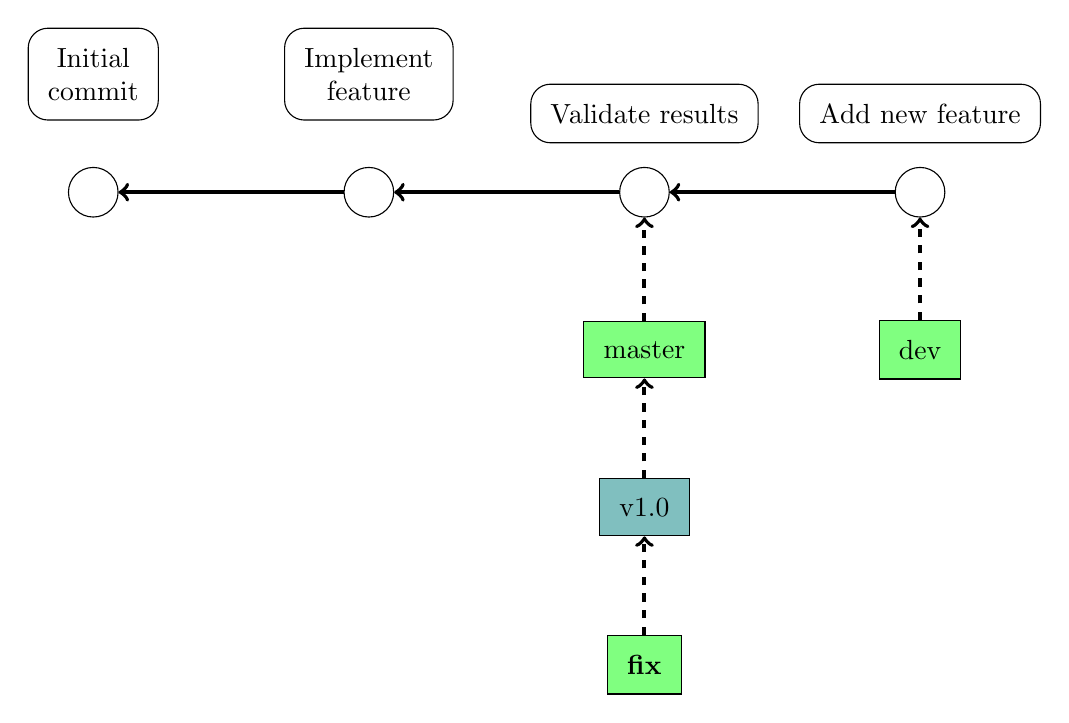
\begin{tikzpicture}[node distance=3.5cm,auto]
    \node[commit] (c1) {\quad};
    \node[commit,right of=c1] (c2) {\quad};
    \node[commit,right of=c2] (c3) {\quad};
    \node[commit,right of=c3] (c4) {\quad};

     \node[branch,below of=c3,node distance=2.0cm] (master) {master};
     \node[tag,below of=master,node distance=2.0cm] (vone) {v1.0};
     \node[branch,below of=vone,node distance=2.0cm] (fix) {\textbf{fix}};
     \node[branch,below of=c4,node distance=2.0cm] (dev) {dev};

     \node[msg,above of=c1,align=center,node distance=1.5cm] (m1) {Initial \\ commit};
     \node[msg,above of=c2,align=center,node distance=1.5cm] (m2) {Implement \\ feature};
     \node[msg,above of=c3] (m3) {Validate results};
     \node[msg,above of=c4] (m4) {Add new feature};

        \path[arrow, <-] (c1) -- (c2);
        \path[arrow, <-] (c2) -- (c3);
        \path[arrow, <-] (c3) -- (c4);
        \path[arrow,dashed,->] (master) -- (c3);
        \path[arrow,dashed,->] (vone) -- (master);
        \path[arrow,dashed,->] (fix) -- (vone);
        \path[arrow,dashed,->] (dev) -- (c4);
  \end{tikzpicture}

  \clearpage

  \centering
  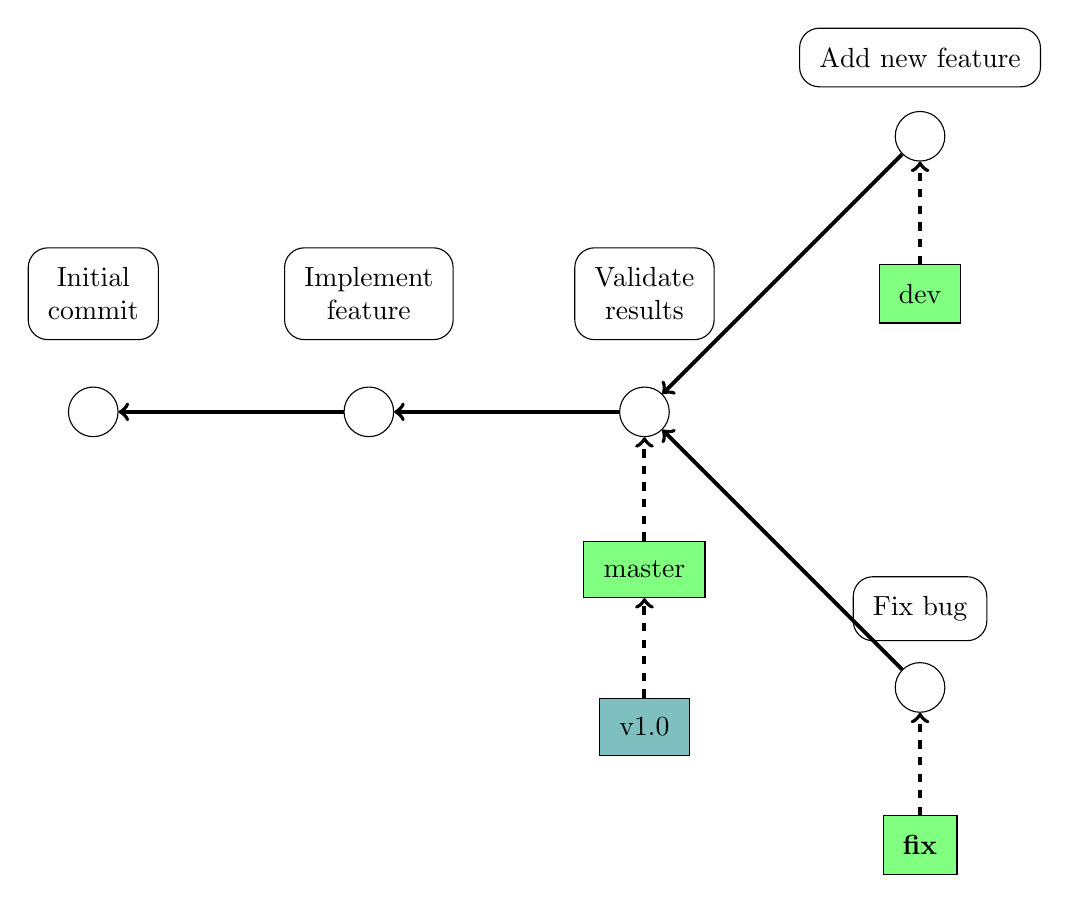
\begin{tikzpicture}[node distance=3.5cm,auto]
    \node[commit] (c1) {\quad};
    \node[commit,right of=c1] (c2) {\quad};
    \node[commit,right of=c2] (c3) {\quad};
    \node[commit,right of=c3,draw=none] (empt) {\quad};
    \node[commit,above of=empt] (c4) {\quad};
    \node[commit,below of=empt] (c5) {\quad};

     \node[branch,below of=c3,node distance=2.0cm] (master) {master};
     \node[tag,below of=master,node distance=2.0cm] (vone) {v1.0};
     \node[branch,below of=c5,node distance=2.0cm] (fix) {\textbf{fix}};
     \node[branch,below of=c4,node distance=2.0cm] (dev) {dev};

     \node[msg,above of=c1,align=center,node distance=1.5cm] (m1) {Initial \\ commit};
     \node[msg,above of=c2,align=center,node distance=1.5cm] (m2) {Implement \\ feature};
     \node[msg,above of=c3,align=center,node distance=1.5cm] (m3) {Validate \\ results};
     \node[msg,above of=c4] (m4) {Add new feature};
     \node[msg,above of=c5] (m5) {Fix bug};

        \path[arrow, <-] (c1) -- (c2);
        \path[arrow, <-] (c2) -- (c3);
        \path[arrow, <-] (c3) -- (c4);
        \path[arrow, <-] (c3) -- (c5);
        \path[arrow,dashed,->] (master) -- (c3);
        \path[arrow,dashed,->] (vone) -- (master);
        \path[arrow,dashed,->] (fix) -- (c5);
        \path[arrow,dashed,->] (dev) -- (c4);
  \end{tikzpicture}

  \clearpage

  \centering
  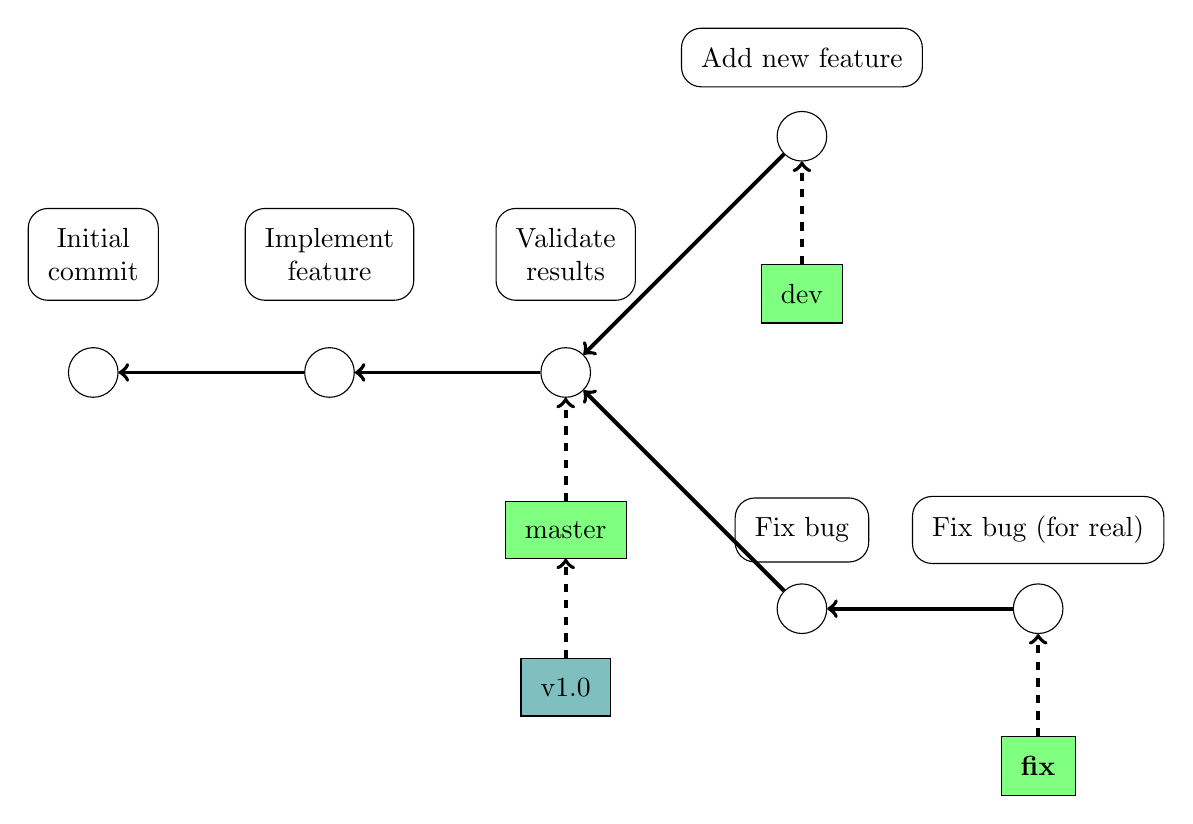
\begin{tikzpicture}[node distance=3.0cm,auto]
    \node[commit] (c1) {\quad};
    \node[commit,right of=c1] (c2) {\quad};
    \node[commit,right of=c2] (c3) {\quad};
    \node[commit,right of=c3,draw=none] (empt) {\quad};
    \node[commit,above of=empt] (c4) {\quad};
    \node[commit,below of=empt] (c5) {\quad};
    \node[commit,right of=c5] (c6) {\quad};

     \node[branch,below of=c3,node distance=2.0cm] (master) {master};
     \node[tag,below of=master,node distance=2.0cm] (vone) {v1.0};
     \node[branch,below of=c6,node distance=2.0cm] (fix) {\textbf{fix}};
     \node[branch,below of=c4,node distance=2.0cm] (dev) {dev};

     \node[msg,above of=c1,align=center,node distance=1.5cm] (m1) {Initial \\ commit};
     \node[msg,above of=c2,align=center,node distance=1.5cm] (m2) {Implement \\ feature};
     \node[msg,above of=c3,align=center,node distance=1.5cm] (m3) {Validate \\ results};
     \node[msg,above of=c4] (m4) {Add new feature};
     \node[msg,above of=c5] (m5) {Fix bug};
     \node[msg,above of=c6] (m6) {Fix bug (for real)};

        \path[arrow, <-] (c1) -- (c2);
        \path[arrow, <-] (c2) -- (c3);
        \path[arrow, <-] (c3) -- (c4);
        \path[arrow, <-] (c3) -- (c5);
        \path[arrow, <-] (c5) -- (c6);
        \path[arrow,dashed,->] (master) -- (c3);
        \path[arrow,dashed,->] (vone) -- (master);
        \path[arrow,dashed,->] (fix) -- (c6);
        \path[arrow,dashed,->] (dev) -- (c4);
  \end{tikzpicture}

  \clearpage

  \centering
  \begin{tikzpicture}[node distance=3.0cm,auto]
    \node[commit] (c1) {\quad};
    \node[commit,right of=c1] (c2) {\quad};
    \node[commit,right of=c2] (c3) {\quad};
    \node[commit,right of=c3,draw=none] (empt) {\quad};
    \node[commit,above of=empt] (c4) {\quad};
    \node[commit,below of=empt] (c5) {\quad};
    \node[commit,right of=c5] (c6) {\quad};

     \node[branch,below of=c6,node distance=2.0cm] (master) {\textbf{master}};
     \node[tag,below of=c3,node distance=2.0cm] (vone) {v1.0};
     \node[branch,below of=c4,node distance=2.0cm] (dev) {dev};

     \node[msg,above of=c1,align=center,node distance=1.5cm] (m1) {Initial \\ commit};
     \node[msg,above of=c2,align=center,node distance=1.5cm] (m2) {Implement \\ feature};
     \node[msg,above of=c3,align=center,node distance=1.5cm] (m3) {Validate \\ results};
     \node[msg,above of=c4] (m4) {Add new feature};
     \node[msg,above of=c5] (m5) {Fix bug};
     \node[msg,above of=c6] (m6) {Fix bug (for real)};

        \path[arrow, <-] (c1) -- (c2);
        \path[arrow, <-] (c2) -- (c3);
        \path[arrow, <-] (c3) -- (c4);
        \path[arrow, <-] (c3) -- (c5);
        \path[arrow, <-] (c5) -- (c6);
        \path[arrow,dashed,->] (master) -- (c6);
        \path[arrow,dashed,->] (vone) -- (c3);
        \path[arrow,dashed,->] (fix) -- (c6);
        \path[arrow,dashed,->] (dev) -- (c4);
  \end{tikzpicture}

  \clearpage

  \centering
  \begin{tikzpicture}[node distance=3.0cm,auto]
    \node[commit] (c1) {\quad};
    \node[commit,right of=c1] (c2) {\quad};
    \node[commit,right of=c2] (c3) {\quad};
    \node[commit,right of=c3,draw=none] (empt) {\quad};
    \node[commit,above of=empt] (c4) {\quad};
    \node[commit,below of=empt] (c5) {\quad};
    \node[commit,right of=c5] (c6) {\quad};

     \node[branch,below of=c6,node distance=2.0cm] (master) {\textbf{master}};
     \node[tag,below of=c3,node distance=2.0cm] (vone) {v1.0};
     \node[tag,below of=master,node distance=2.0cm] (voneone) {v1.1};
     \node[branch,below of=c4,node distance=2.0cm] (dev) {dev};

     \node[msg,above of=c1,align=center,node distance=1.5cm] (m1) {Initial \\ commit};
     \node[msg,above of=c2,align=center,node distance=1.5cm] (m2) {Implement \\ feature};
     \node[msg,above of=c3,align=center,node distance=1.5cm] (m3) {Validate \\ results};
     \node[msg,above of=c4] (m4) {Add new feature};
     \node[msg,above of=c5] (m5) {Fix bug};
     \node[msg,above of=c6] (m6) {Fix bug (for real)};

        \path[arrow, <-] (c1) -- (c2);
        \path[arrow, <-] (c2) -- (c3);
        \path[arrow, <-] (c3) -- (c4);
        \path[arrow, <-] (c3) -- (c5);
        \path[arrow, <-] (c5) -- (c6);
        \path[arrow,dashed,->] (master) -- (c6);
        \path[arrow,dashed,->] (vone) -- (c3);
        \path[arrow,dashed,->] (voneone) -- (master);
        \path[arrow,dashed,->] (fix) -- (c6);
        \path[arrow,dashed,->] (dev) -- (c4);
  \end{tikzpicture}

  \clearpage

  \centering
  \begin{tikzpicture}[node distance=3.0cm,auto]
    \node[commit] (c1) {\quad};
    \node[commit,right of=c1] (c2) {\quad};
    \node[commit,right of=c2] (c3) {\quad};
    \node[commit,right of=c3,draw=none] (empt) {\quad};
    \node[commit,above of=empt] (c4) {\quad};
    \node[commit,below of=empt] (c5) {\quad};
    \node[commit,right of=c5] (c6) {\quad};
    \node[commit,right of=c4] (c7) {\quad};

     \node[branch,below of=c6,node distance=2.0cm] (master) {master};
     \node[tag,below of=c3,node distance=2.0cm] (vone) {v1.0};
     \node[tag,below of=master,node distance=2.0cm] (voneone) {v1.1};
     \node[branch,below of=c7,node distance=2.0cm] (dev) {\textbf{dev}};

     \node[msg,above of=c1,align=center,node distance=1.5cm] (m1) {Initial \\ commit};
     \node[msg,above of=c2,align=center,node distance=1.5cm] (m2) {Implement \\ feature};
     \node[msg,above of=c3,align=center,node distance=1.5cm] (m3) {Validate \\ results};
     \node[msg,above of=c4,align=center,node distance=1.5cm] (m4) {Add \\ new \\ feature};
     \node[msg,above of=c5,align=center,node distance=1.5cm] (m5) {Fix \\ bug};
     \node[msg,above of=c6,align=center,node distance=1.5cm] (m6) {Fix \\ bug \\ (for real)};
     \node[msg,above of=c7] (m7) {Test code};

        \path[arrow, <-] (c1) -- (c2);
        \path[arrow, <-] (c2) -- (c3);
        \path[arrow, <-] (c3) -- (c4);
        \path[arrow, <-] (c3) -- (c5);
        \path[arrow, <-] (c5) -- (c6);
        \path[arrow, <-] (c4) -- (c7);
        \path[arrow,dashed,->] (master) -- (c6);
        \path[arrow,dashed,->] (vone) -- (c3);
        \path[arrow,dashed,->] (voneone) -- (master);
        \path[arrow,dashed,->] (fix) -- (c6);
        \path[arrow,dashed,->] (dev) -- (c7);
  \end{tikzpicture}

  \clearpage

  \centering
  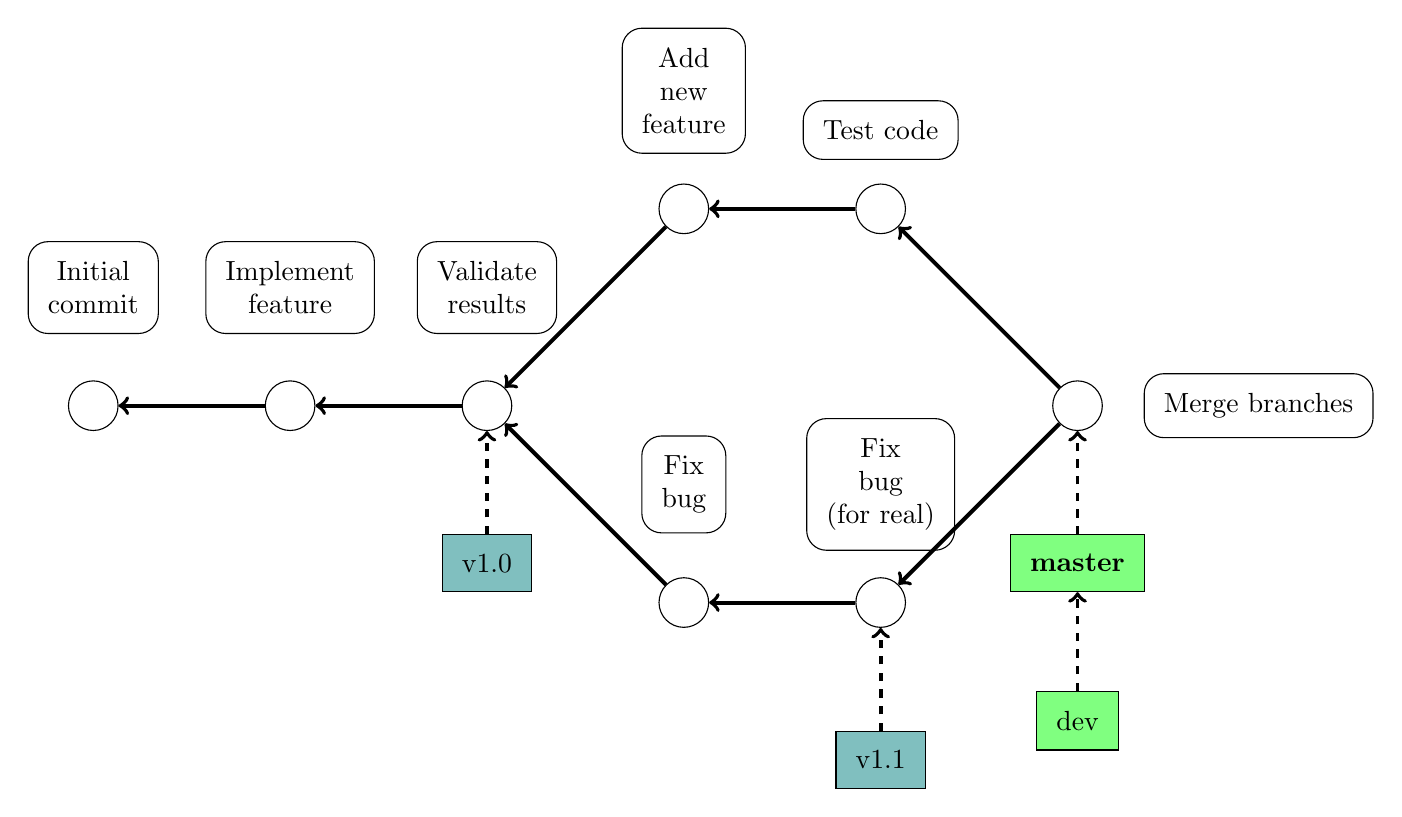
\begin{tikzpicture}[node distance=2.5cm,auto]
    \node[commit] (c1) {\quad};
    \node[commit,right of=c1] (c2) {\quad};
    \node[commit,right of=c2] (c3) {\quad};
    \node[commit,right of=c3,draw=none] (empt) {\quad};
    \node[commit,above of=empt] (c4) {\quad};
    \node[commit,below of=empt] (c5) {\quad};
    \node[commit,right of=c5] (c6) {\quad};
    \node[commit,right of=c4] (c7) {\quad};
    \node[commit,right of=empt,node distance=5cm] (c8) {\quad};

     \node[branch,below of=c8,node distance=2.0cm] (master) {\textbf{master}};
     \node[tag,below of=c3,node distance=2.0cm] (vone) {v1.0};
     \node[tag,below of=c6,node distance=2.0cm] (voneone) {v1.1};
     \node[branch,below of=master,node distance=2.0cm] (dev) {dev};

     \node[msg,above of=c1,align=center,node distance=1.5cm] (m1) {Initial \\ commit};
     \node[msg,above of=c2,align=center,node distance=1.5cm] (m2) {Implement \\ feature};
     \node[msg,above of=c3,align=center,node distance=1.5cm] (m3) {Validate \\ results};
     \node[msg,above of=c4,align=center,node distance=1.5cm] (m4) {Add \\ new \\ feature};
     \node[msg,above of=c5,align=center,node distance=1.5cm] (m5) {Fix \\ bug};
     \node[msg,above of=c6,align=center,node distance=1.5cm] (m6) {Fix \\ bug \\ (for real)};
     \node[msg,above of=c7] (m7) {Test code};
     \node[msg,right of=c8,node distance=2.3cm] (m8) {Merge branches};

        \path[arrow, <-] (c1) -- (c2);
        \path[arrow, <-] (c2) -- (c3);
        \path[arrow, <-] (c3) -- (c4);
        \path[arrow, <-] (c3) -- (c5);
        \path[arrow, <-] (c5) -- (c6);
        \path[arrow, <-] (c4) -- (c7);
        \path[arrow, <-] (c7) -- (c8);
        \path[arrow, <-] (c6) -- (c8);
        \path[arrow,dashed,->] (master) -- (c8);
        \path[arrow,dashed,->] (vone) -- (c3);
        \path[arrow,dashed,->] (voneone) -- (c6);
        \path[arrow,dashed,->] (dev) -- (master);
  \end{tikzpicture}

  \clearpage

  \centering
  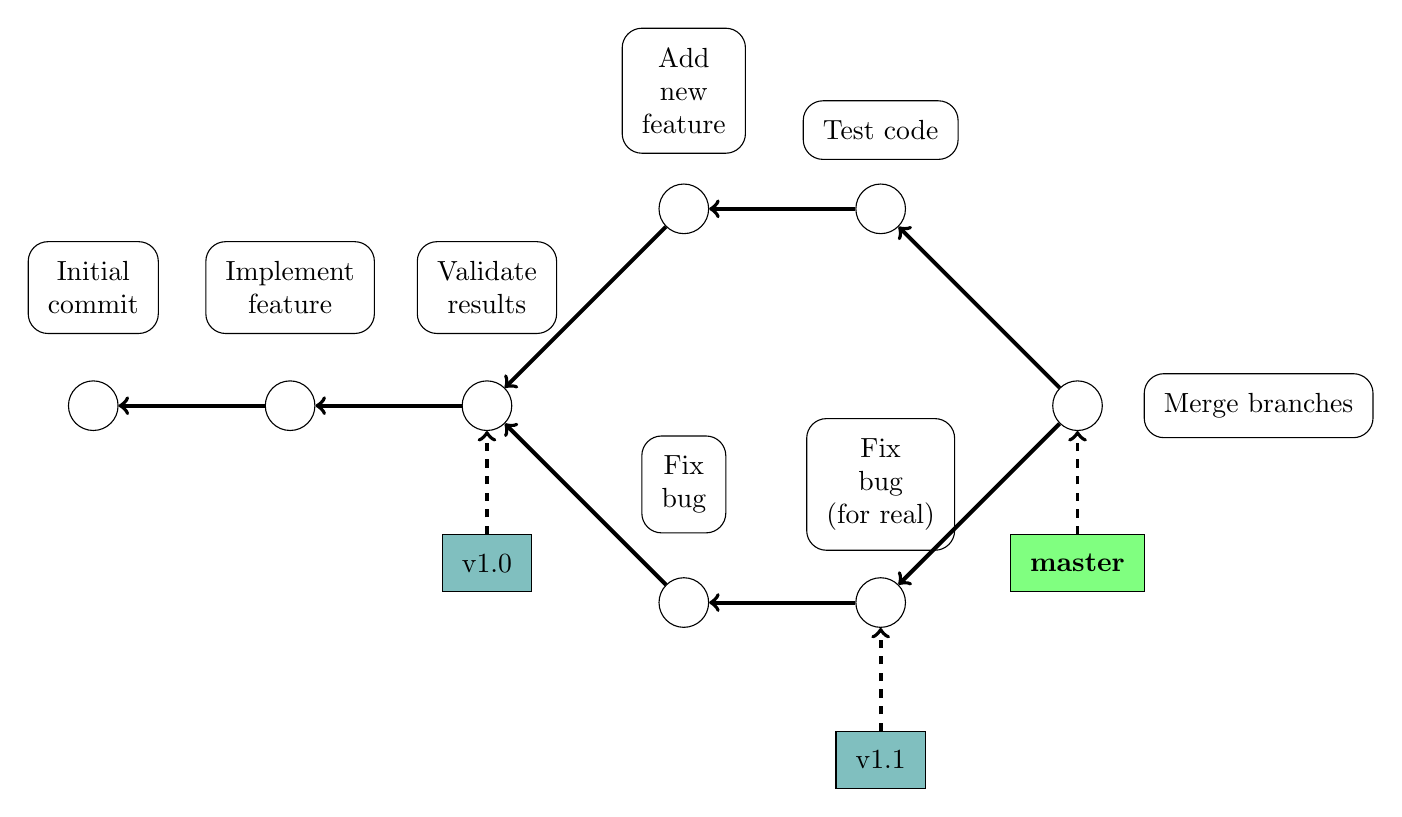
\begin{tikzpicture}[node distance=2.5cm,auto]
    \node[commit] (c1) {\quad};
    \node[commit,right of=c1] (c2) {\quad};
    \node[commit,right of=c2] (c3) {\quad};
    \node[commit,right of=c3,draw=none] (empt) {\quad};
    \node[commit,above of=empt] (c4) {\quad};
    \node[commit,below of=empt] (c5) {\quad};
    \node[commit,right of=c5] (c6) {\quad};
    \node[commit,right of=c4] (c7) {\quad};
    \node[commit,right of=empt,node distance=5cm] (c8) {\quad};

     \node[branch,below of=c8,node distance=2.0cm] (master) {\textbf{master}};
     \node[tag,below of=c3,node distance=2.0cm] (vone) {v1.0};
     \node[tag,below of=c6,node distance=2.0cm] (voneone) {v1.1};

     \node[msg,above of=c1,align=center,node distance=1.5cm] (m1) {Initial \\ commit};
     \node[msg,above of=c2,align=center,node distance=1.5cm] (m2) {Implement \\ feature};
     \node[msg,above of=c3,align=center,node distance=1.5cm] (m3) {Validate \\ results};
     \node[msg,above of=c4,align=center,node distance=1.5cm] (m4) {Add \\ new \\ feature};
     \node[msg,above of=c5,align=center,node distance=1.5cm] (m5) {Fix \\ bug};
     \node[msg,above of=c6,align=center,node distance=1.5cm] (m6) {Fix \\ bug \\ (for real)};
     \node[msg,above of=c7] (m7) {Test code};
     \node[msg,right of=c8,node distance=2.3cm] (m8) {Merge branches};

        \path[arrow, <-] (c1) -- (c2);
        \path[arrow, <-] (c2) -- (c3);
        \path[arrow, <-] (c3) -- (c4);
        \path[arrow, <-] (c3) -- (c5);
        \path[arrow, <-] (c5) -- (c6);
        \path[arrow, <-] (c4) -- (c7);
        \path[arrow, <-] (c7) -- (c8);
        \path[arrow, <-] (c6) -- (c8);
        \path[arrow,dashed,->] (master) -- (c8);
        \path[arrow,dashed,->] (vone) -- (c3);
        \path[arrow,dashed,->] (voneone) -- (c6);
  \end{tikzpicture}

  \clearpage

  \centering
  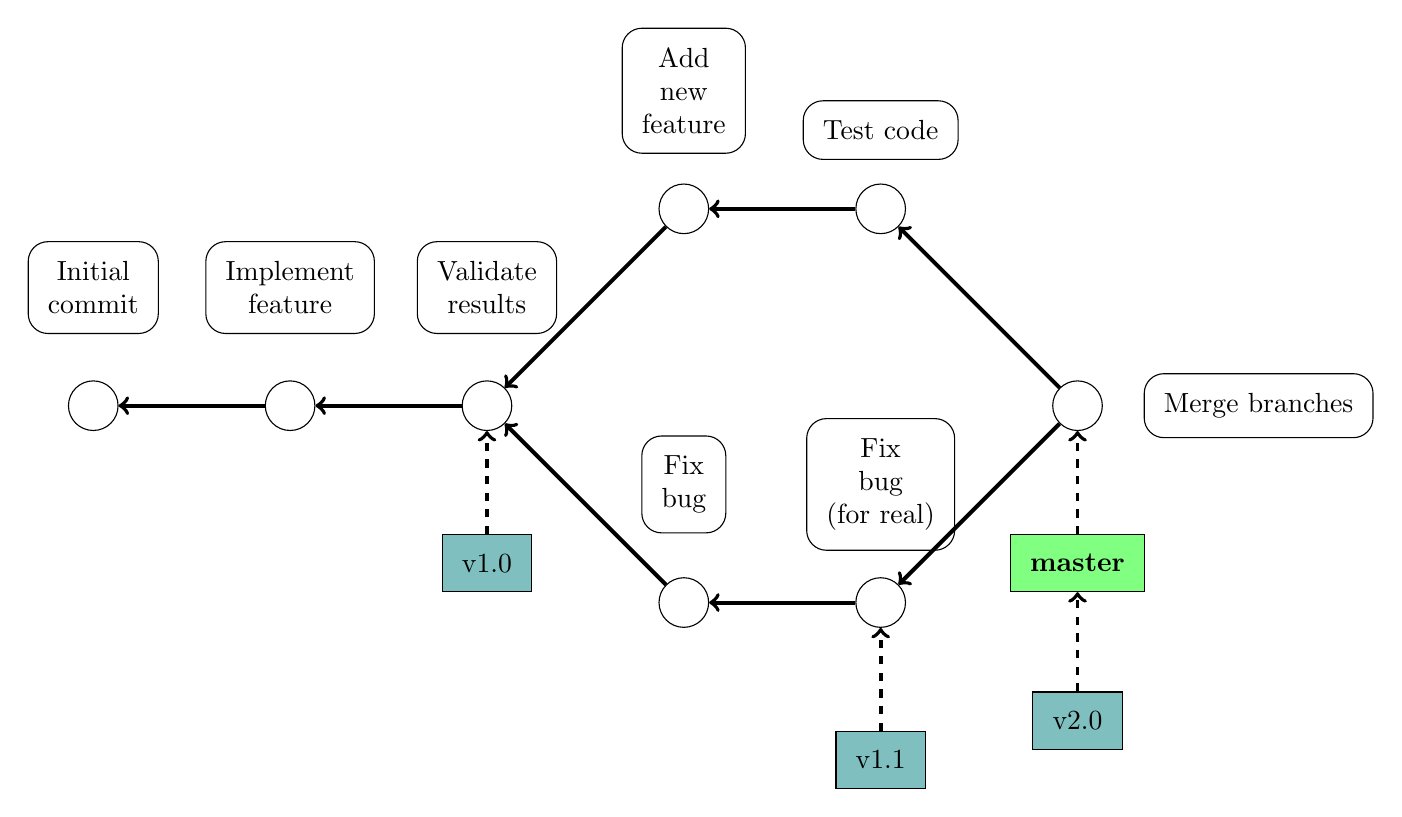
\begin{tikzpicture}[node distance=2.5cm,auto]
    \node[commit] (c1) {\quad};
    \node[commit,right of=c1] (c2) {\quad};
    \node[commit,right of=c2] (c3) {\quad};
    \node[commit,right of=c3,draw=none] (empt) {\quad};
    \node[commit,above of=empt] (c4) {\quad};
    \node[commit,below of=empt] (c5) {\quad};
    \node[commit,right of=c5] (c6) {\quad};
    \node[commit,right of=c4] (c7) {\quad};
    \node[commit,right of=empt,node distance=5cm] (c8) {\quad};

     \node[branch,below of=c8,node distance=2.0cm] (master) {\textbf{master}};
     \node[tag,below of=c3,node distance=2.0cm] (vone) {v1.0};
     \node[tag,below of=c6,node distance=2.0cm] (voneone) {v1.1};
     \node[tag,below of=master,node distance=2.0cm] (vtwo) {v2.0};

     \node[msg,above of=c1,align=center,node distance=1.5cm] (m1) {Initial \\ commit};
     \node[msg,above of=c2,align=center,node distance=1.5cm] (m2) {Implement \\ feature};
     \node[msg,above of=c3,align=center,node distance=1.5cm] (m3) {Validate \\ results};
     \node[msg,above of=c4,align=center,node distance=1.5cm] (m4) {Add \\ new \\ feature};
     \node[msg,above of=c5,align=center,node distance=1.5cm] (m5) {Fix \\ bug};
     \node[msg,above of=c6,align=center,node distance=1.5cm] (m6) {Fix \\ bug \\ (for real)};
     \node[msg,above of=c7] (m7) {Test code};
     \node[msg,right of=c8,node distance=2.3cm] (m8) {Merge branches};

        \path[arrow, <-] (c1) -- (c2);
        \path[arrow, <-] (c2) -- (c3);
        \path[arrow, <-] (c3) -- (c4);
        \path[arrow, <-] (c3) -- (c5);
        \path[arrow, <-] (c5) -- (c6);
        \path[arrow, <-] (c4) -- (c7);
        \path[arrow, <-] (c7) -- (c8);
        \path[arrow, <-] (c6) -- (c8);
        \path[arrow,dashed,->] (master) -- (c8);
        \path[arrow,dashed,->] (vone) -- (c3);
        \path[arrow,dashed,->] (voneone) -- (c6);
        \path[arrow,dashed,->] (vtwo) -- (master);
  \end{tikzpicture}

  \clearpage

  \centering
  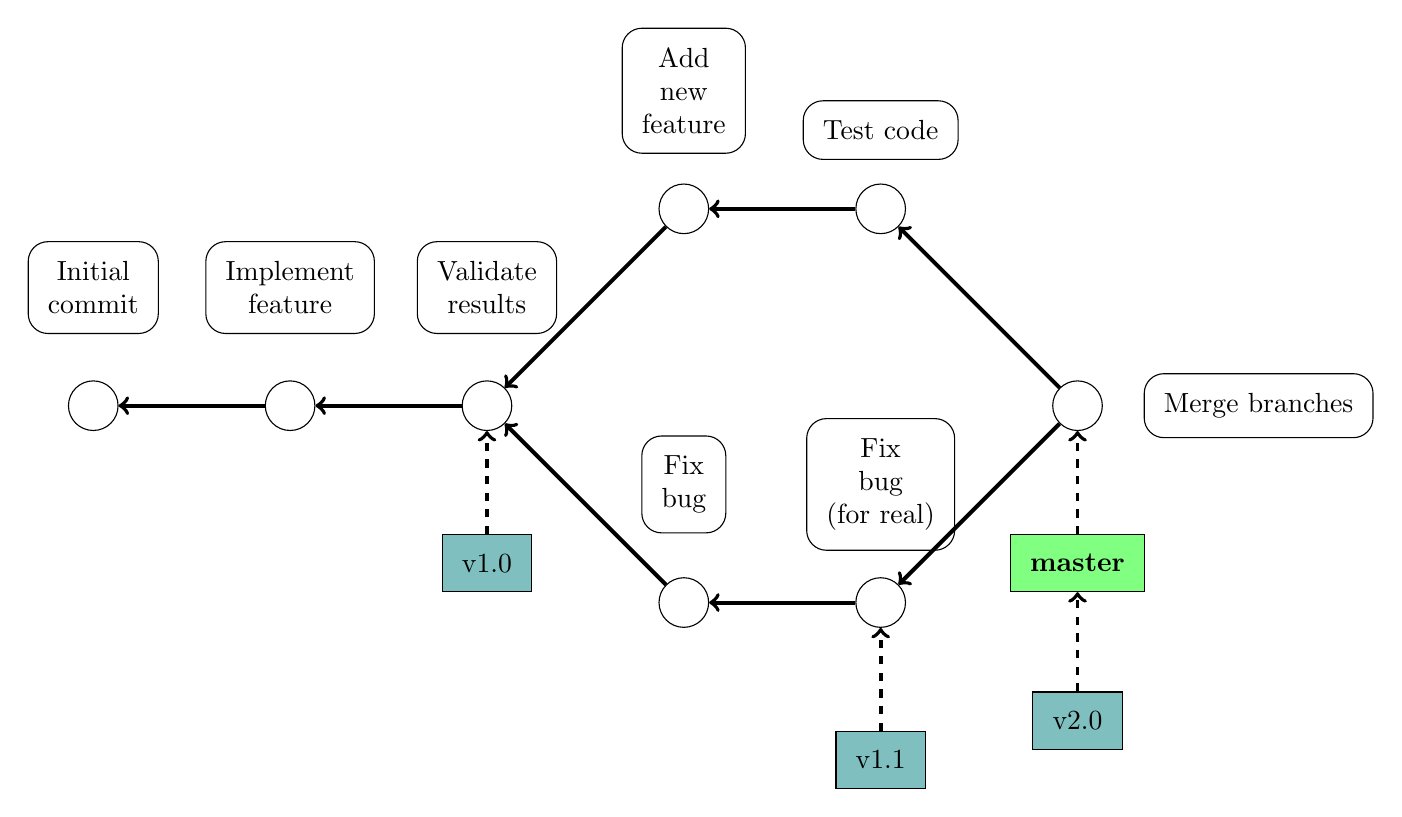
\begin{tikzpicture}[node distance=2.5cm,auto]
    \node[commit] (c1) {\quad};
    \node[commit,right of=c1] (c2) {\quad};
    \node[commit,right of=c2] (c3) {\quad};
    \node[commit,right of=c3,draw=none] (empt) {\quad};
    \node[commit,above of=empt] (c4) {\quad};
    \node[commit,below of=empt] (c5) {\quad};
    \node[commit,right of=c5] (c6) {\quad};
    \node[commit,right of=c4] (c7) {\quad};
    \node[commit,right of=empt,node distance=5cm] (c8) {\quad};

     \node[branch,below of=c8,node distance=2.0cm] (master) {\textbf{master}};
     \node[tag,below of=c3,node distance=2.0cm] (vone) {v1.0};
     \node[tag,below of=c6,node distance=2.0cm] (voneone) {v1.1};
     \node[tag,below of=master,node distance=2.0cm] (vtwo) {v2.0};

     \node[msg,above of=c1,align=center,node distance=1.5cm] (m1) {Initial \\ commit};
     \node[msg,above of=c2,align=center,node distance=1.5cm] (m2) {Implement \\ feature};
     \node[msg,above of=c3,align=center,node distance=1.5cm] (m3) {Validate \\ results};
     \node[msg,above of=c4,align=center,node distance=1.5cm] (m4) {Add \\ new \\ feature};
     \node[msg,above of=c5,align=center,node distance=1.5cm] (m5) {Fix \\ bug};
     \node[msg,above of=c6,align=center,node distance=1.5cm] (m6) {Fix \\ bug \\ (for real)};
     \node[msg,above of=c7] (m7) {Test code};
     \node[msg,right of=c8,node distance=2.3cm] (m8) {Merge branches};

        \path[arrow, <-] (c1) -- (c2);
        \path[arrow, <-] (c2) -- (c3);
        \path[arrow, <-] (c3) -- (c4);
        \path[arrow, <-] (c3) -- (c5);
        \path[arrow, <-] (c5) -- (c6);
        \path[arrow, <-] (c4) -- (c7);
        \path[arrow, <-] (c7) -- (c8);
        \path[arrow, <-] (c6) -- (c8);
        \path[arrow,dashed,->] (master) -- (c8);
        \path[arrow,dashed,->] (vone) -- (c3);
        \path[arrow,dashed,->] (voneone) -- (c6);
        \path[arrow,dashed,->] (vtwo) -- (master);
  \end{tikzpicture}
\end{document}